\chapter{Software Development at HubSpot}
Software development has been a core part of HubSpot since day one. As such, the overall development process and methodology has undergone several iterations. Critically, at each iteration, the development process is reevaluated and the experience gained over the past number of years is capitalized upon. This has led to a streamlined and simple development process which is easy to learn, allowing both new hires and temporary interns to get up to speed quickly. HubSpot also has several \textit{platform} teams solely dedicated to providing easy to use integrations of powerful tools which can be cumbersome to configure on a per project basis. These teams contribute to what's known as the overall \textit{platform as a service (PaaS)}. Product development teams can then use this platform to get access to these powerful tools, without needing to spend time on configuration.

As all of HubSpot is built on the same technology stack and all projects adhere to a common project structure, any developer can drop into any project owned by another team and immediately know where to search for what they are looking for. This has the direct benefits of allowing engineers to fix bugs they encounter when using other teams' projects. One of HubSpot's core beliefs when it comes to software engineering is that everyone should contribute what they can, instead of passing the blame to other teams. Most engineers are busy with new tasks and challenges and fixing a bug in code that belongs to a fellow engineer is substantially more productive for \textbf{both} teams than filing an issue and waiting for it to be resolved. 

\section{Technologies in use at HubSpot}
As discussed, all of HubSpot is built using a set of technologies. This set of technologies is continuously growing as needs change and as new technologies become available. Typically, any given team and/or project will use a subset of the technologies on offer. This section outlines some of the core technologies used by the \team{} team. 
\subsection{Java 8}
Java 8 is the second to newest release of Java. Java as a language has been around since the mid 1990s and has been under continuous development since then. As such, it has become a very stable and reliable language, used by nine million developers worldwide \cite{java9Million}. At HubSpot, Java 8 is used for the development of all backend services. The architecture employed is one of micro-services. This allows for rapid development and deployment of many loosely coupled services. The services are extremely modular and are often used by a variety of teams and projects. 

Java is an object oriented language which provides a variety of concepts to aid in system design. Classically, the core of object oriented programming is that entities (objects) should model one \textit{real} entity and one only. Clients can then use these objects in their own classes, abstracting away all the complex implementation logic of the imported class from the client. Any information required by the object can be encapsulated within the object itself allowing the object to provide a simple interface to its users, consisting of a number of methods, which if named correctly, provide a succinct description of what the method does which lines up exactly with what the client thinks the method should do.

Java 8 was released in March 2014 and provides several new and extremely powerful features, many of which are used on a daily basis at HubSpot. Aside from all the core functionality contained in Java, a subset of the most interesting and useful features it provides are outlined below.

%% Lambdas
\sneaktitle{Lambda Expressions}
Often times it is useful to create classes which wrap a piece of logic or code. Similarly, systems often require the execution of a piece of code in response to a certain event (e.g. running some code in response to a mouse click). Traditionally in java this was accomplished by writing a manual \textit{functional interface}. These functional interfaces were simple interfaces which provided a contract containing a single method. The class in question can then be passed an instance of an object which implements the functional interface and can thus invoke the method defined in the interface when appropriate. An example of this using traditional Java is outlined in \refcode{lst:noLambda} which contains code for a button that can be clicked and can have on-click methods associated with it. Prior to Java 8, this code was cumbersome to write requiring a custom interface to be created, implemented by a concrete class and its implementation instantiated and passed to the class which manages the events. 

\lstinputlisting[
  caption={onClick Listener without Lambda Expression},
  label={lst:noLambda},
  style=javaStyle
  ]{code/technologies/NoLambda.java}

This code can be written in a much more concise form by using Java 8's new lambda expressions. The JDK now provides the most common functional interfaces which can be used in place of custom functional interfaces. For example the \java{Consumer<T>} functional interface, defines a single \java{accept} function which takes an argument of type \java{T} and returns nothing (it \textit{consumes} the argument), which is exactly what the \java{OnClickRunner} in \refcode{lst:noLambda} defined. The \java{Button} class can be refactored to use a \java{Consumer<String>}, allowing the logic of the \java{OnClickRunner} to be directly specified through a lambda expression. An example of this is shown in \refcode{lst:withLambda} and the lambda expression can be seen on line 16.
\vfill

\lstinputlisting[
  caption={onClick Listener with Lambda Expression},
  label={lst:withLambda},
  style=javaStyle
  ]{code/technologies/Lambda.java}

As seen in \refcode{lst:withLambda}, the use of lambda expressions greatly simplifies the code. Several functional interfaces exist to enable the use of lambda expressions for functions with differing signatures. For example \java{BiConsumer<T, U>} represents a function which takes two arguments of type \java{T} and \java{U} respectively and returns nothing, or the more generic \java{Function<T, R>} which takes an argument of type \java{T} and returns a value of type \java{R}.

%% Streams
\sneaktitle{Streams}
Another extremely powerful feature of Java 8 is the new Stream API. This allows for the bulk processing of collections through map/reduce like operations. Performing arbitrary data manipulation on a collection of Java objects is extremely common. Typically, this could be accomplished using a simple loop. However this often requires the introduction of several local variables which can add excessive noise to code. Of course, some operations are still better suited to a simple loop, particularly if the data transformation function has side effects, in which case it is impossible to use streams. However it is widely considered good practice to minimize side effects of functions in order to maintain simplicity and making heavy use of streams is a great way to remind developers not to introduce side effects and to in general, minimize the amount of state required by a class. The Java 8 Stream API is fluent, allowing for arbitrarily complex stream operations to be chained together. Streams are also evaluated lazily, minimizing the amount of work to be done and can be parallelized internally by the API, providing excellent performance. The Java 8 Stream API consists of three types of operations: 

\begin{labeling}{Intermediate Operations  }
	\item [Initial stream call] The \java{stream()} call can be invoked on any object that implements the \java{Collection} interface. This call returns a \java{Stream<T>} (where \java{T} is the type of the objects in the collection) allowing subsequent intermediate and terminal operations to be invoked on the returned stream.
	\item [Intermediate Operations  ] These are the operations which perform the data transformation. There are a variety of intermediate operations provided such as \java{sort} which sorts the objects in the stream, \java{filter} which filters objects in the stream according to some predicate and \java{map} which maps an arbitrary function over each object in the stream. As mentioned, the Stream API is fluent, meaning multiple intermediate operations can be chained together (for example filtering the objects and then sorting them).
	\item [Terminal Operations] The is the final operation which describes how the data should be reduced to a single object (which may be a collection). Common terminal operations are \java{max} which returns the maximum of the objects in the stream, \java{findFirst} which returns the first object the stream encounters that matches a given predicate and \java{collect} which defines how the objects in the stream should be collected into a collection (for example collecting the objects into a set would remove any duplicates)
\end{labeling}

Comparing \refcode{lst:withoutStreams} and \refcode{lst:withStreams}, the clarity of the code produced using the Streams API can be seen. The code listings shows two approaches to a piece of logic which returns the length of each of the strings (in ascending order), without white space, and which don't contain the word \textit{owl}. Although this is a toy example, several benefits of the Streams API can be seen. The code using streams (\refcode{lst:withStreams}) reads like the steps of a recipe, clearly stating what is performed at each step. However the code using the traditional \java{for} loop (\refcode{lst:withoutStreams}) requires \java{if} statements and redundant local variables, distracting the programmer from the core steps of the algorithm. Streams also provide the benefits of immutability and parallelism for free.

\lstinputlisting[
  caption={Batch Processing without Streams},
  label={lst:withoutStreams},
  style=javaStyle
  ]{code/technologies/NoStreams.java}

\lstinputlisting[
  caption={Batch Processing with Streams},
  label={lst:withStreams},
  style=javaStyle
  ]{code/technologies/Streams.java}


%% Completable Futures
\sneaktitle{Completable Futures}
Asynchronous programming is present in most modern systems. In the early days of Java, this was accomplished by the JDK through abstractions at the thread level. This required careful tracking of the state of threads by the programmer. Concurrent programs are incredibly difficult to reason about and thus concurrency is one of the most challenging aspects of modern software engineering and is the source of a huge number of bugs. However, the benefits of concurrent programming are extremely obvious, essentially making it a necessity in modern systems. Thus, any abstractions that can aid in reducing the number of things a programmer must keep track of will be beneficial. In Java 8's case, this abstraction is the \java{CompletableFuture} API. This API allows for programmers to perform asynchronous tasks by specifying a \java{Supplier<U>}, a function which takes no arguments and returns (supplies) a value of type \java{U}, which will return a value at some point in the future. Thus, what's returned from this call is not an instance of type \java{U}, but a \java{CompletableFuture<U>}, that is, an object that at some point in the future will contain an instance of type \java{U} (provided no errors occur). 

The programmer may also specify an \java{Executor} \cite{javaExecutor} which is essentially an object (e.g. threadpool) capable of running tasks on a thread other than the thread in the current context. If no \java{Executor} is specified, the task is automatically submitted to Java's work stealing \java{ForkJoinPool} \cite{javaForkJoinPool}. 

The API provides a simple \java{get} method for blocking until the return value is present (or throws an exception). More interestingly however, it also provides several methods to specify subsequent processing of the return value when it returns, allowing the program to continue doing useful work while waiting on the result. A subset of these methods are the following \cite{javaCfArticle}:

\begin{labeling}{thenCompose}
	\item [thenApply] This method is used to supply a function that should be run upon completion of the underlying \java{CompletableFuture}. The result of the \java{CompletableFuture} will be passed as the sole argument to this function. This function is free to return any type and in doing so, sets the type associated with the underlying \java{CompletableFuture}. 
	\item [thenCompose] This method is very similar to \java{thenApply} except it is used when the desired function to be run is also asynchronous (that is, it too returns a \java{CompletableFuture}). This behavior could technically also be handled by \java{thenApply} (as it is free to return any value), but this would cause the return type of the parent \java{CompletableFuture} to itself be a \java{CompletableFuture}. The benefit of \java{thenCompose} is that it contains logic to unwrap this nested \java{CompletableFuture}, allowing the return type of the parent to remain a \java{CompletableFuture<T>} even if the function passed to \java{thenCompose} itself returns a \java{CompletableFuture<T>}.
	\item [thenAccept] This method is used when the return type of the \java{CompletableFuture} only needs to be used in the registered callback and is not used outside of the supplied function. As such, this method takes a \java{Consumer<T>} as its argument, that is, a function which takes \java{T} as a parameter and does not return anything.  
\end{labeling}

Finally, all these methods contain corresponding methods in which an \java{Executor} is also specified. This allows the callbacks to be run on the specified \java{Executor} (thread pool).


\subsection{Guice - Dependency Injection}\label{sec:guice}
Google's Guice \cite{guice} is a dependency injection framework for Java. Dependency injection is a software pattern which abstracts away the actual construction (instantiation) of objects from the user. As a system grows and abstractions are built atop of one and other, simply instantiating an object can be come tedious and difficult. Traditionally, in order to instantiate an object, all of its unconditionally required dependencies must be passed to the constructor of the object. Otherwise, the object could be left in an inconsistent state. Thus, in order to instantiate an object \java{O}, all its dependencies, for example \java{X, Y and Z} must be provided to \java{O}'s constructor. Thus, the client of \java{O} must first instantiate instances of \java{X, Y and Z} before it can use \java{O}. However \java{X} may have its own set of dependencies and the problem simply gets worse and worse. An example of the difficulties this can cause (based on the example in Guice's documentation \cite{guiceDocs}) is shown in \refcode{lst:noDI}. The code shown has to recursively create each of the dependencies for each of its dependencies which can quickly get out of hand for large systems.

\lstinputlisting[
  caption={Pizza Ordering Service without Dependency Injection},
  label={lst:noDI},
  style=javaStyle
  ]{code/technologies/NoDI.java}

Traditionally, this problem was somewhat helped (but not entirely solved) by the using the factory pattern \cite{factoryMethodPattern}. Depending on the implementation, this can ease the pain of getting access to objects the client depends on, by allowing the factory to contain the logic for the instantiation of the class' dependencies. However this still requires the manual implementation of the factory classes themselves, leaving much to be desired.


Dependency injection solves this problem by allowing fully formed instances of dependencies (e.g. a \java{PaypPalCustomerBiller}) to be \textit{passed} to the client, removing the need for the client to instantiate the object themselves. Client's simply ask for their dependencies to be injected into their constructor. Guice provides this functionality by simply annotating the constructor with the \java{@Inject} annotation. This (along with some other boilerplate) informs Guice that this class should have its dependencies injected into the class' constructor. Guice accomplishes this by building an arbitrarily complex dependency graph at run time. When a class needs a certain dependency, the graph can be examined in order to figure out how to instantiate that dependency. 

However Guice does need a starting point - dependencies can't just be injected for every single class without providing some initial classes in which to build upon. In the example above, these base classes would be the \java{SqlCredentials} and \java{PayPalCredentials} classes. These classes should not have any injected dependencies. In this example these could simply read the credentials needed from a file. Guice allows us to add vertices to the dependency graph by \textit{providing} objects using the \java{@Provides} annotation. Thus, both \java{SqlCredentials} and \java{PayPalCredentials} would need to be provided using \java{@Provides}. The resulting object graph from the code above is show in \reffig{fig:depGraph} - notice the classes at the bottom of the hierarchy are \textbf{provided}. 

\begin{figure}[H]
      \centering
      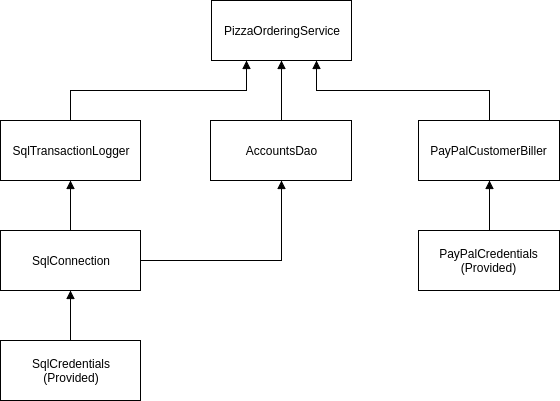
\includegraphics[width=0.7\textwidth]{renders/DependencyInjection.png}
      \caption{Dependency Graph Built by Guice}
      \label{fig:depGraph}
\end{figure}

This leads to extremely simple code for the \java{PizzaOrderingService} in which the logic is entirely separated from the dependency management.

\lstinputlisting[
  caption={Pizza Ordering Service with Dependency Injection},
  label={lst:DI},
  style=javaStyle
  ]{code/technologies/DI.java}

Aside from abstracting away the dependency instantiation, dependency injection also has the added benefit in that all of a class' dependencies become part of the class' constructor signature. There are no required dependencies that are buried within the implementation logic. This makes the code much simpler to test. The \java{PayPalCustomerBiller} used by the class is essentially hardwired into the code that does not use dependency injection (\refcode{lst:noDI}), meaning there is no way to test this class without actually billing a (fake) customer. However as the \java{PayPalCustomerBiller} used by the dependency injected code (\refcode{lst:DI}) is injected into the constructor, a mock of this object (which skips the actual billing, but returns results as if it actually billed a customer) can be passed to the class and used for testing purposes.   

\subsection{Immutables - Immutability for Java}
Immutability is a programming paradigm in which once an object is created, it may never been changed. At first glance this sounds like a bad idea which will result in redundant object creation, but the positives strongly outweigh the negatives. The primary benefit of immutability is that the programmer is \textbf{guaranteed} that any object they hold a reference to, will never be changed. This concept is closely tied to the concept of writing \textit{pure} functions. These are functions which have no external side effects. That is, they take in arguments and return a value, but do not change the input arguments (or any other state contained in the program) in any way. 

These benefits are best highlighted through sample code. Consider the case of a simple website where each login attempt by a user should be logged to a database table in order to detect a hacker trying to crack a password by repeatedly trying to login as the same user. For obvious reasons, this table should not store the user's password (in case of real login attempts), so this should be omitted from the object being logged to the database. An example \java{LoginRequest} is shown in \refcode{lst:loginRequest}. A \java{LoginAttemptLogger} class is written to handle logging these attempts to the database and is shown in \refcode{lst:loginAttemptLogger}. The \java{logLoginAttempt} method handles stripping the password from the \java{LoginRequest} and writing it to the database. 

\lstinputlisting[
  caption={An Example \java{LoginRequest}},
  label={lst:loginRequest},
  style=javaStyle
  ]{code/technologies/immutability/LoginRequest.java}

\lstinputlisting[
  caption={An Example \java{LoginAttemptLogger} Implementation},
  label={lst:loginAttemptLogger},
  style=javaStyle
  ]{code/technologies/immutability/LoginAttemptLogger.java}

However this style of code is a recipe for disaster. The \java{LoginRequest} is \textit{mutable} and the \java{logLoginAttempt} method contains a side effect in that it sets the password of the \java{LoginRequest} to an empty string. Some perfectly reasonable client code is shown in \refcode{lst:clientLoginCode} in which the client logs the login request to the database and subsequently tries to log in. In this case, no user will ever be able to login as all the passwords of the login requests are always mutated to be an empty string. Thus, having \java{LoginRequest} as a mutable object causes a critical bug that will not be caught until runtime. The client login code may check and find that the \java{LoginRequest} contains a password prior to logging the login attempt to the database. However when it goes to finally login, it never will.

\lstinputlisting[
  caption={Perfectly Reasonable Client Login Code},
  label={lst:clientLoginCode},
  style=javaStyle
  ]{code/technologies/immutability/ClientLogin.java}

The solution to this problem is to create a new \java{LoginRequest} without the user's password and log that to the database. This can be done inside of the client login code (defensive copying) before passing the \java{LoginReuqest} to the \java{logLoginAttempt}. However if mutators are provided, it is extremely likely that they will be used somewhere in the code. Thus, the best solution is simply to not provide them at all - make the object entirely immutable. This in turn requires some clunky code inside of the client login method (see \refcode{lst:clunkyImmutableClient}), but avoids the issue caused by the side effect of \java{logLoginAttempt}. 

\lstinputlisting[
  caption={Logically Correct Login Code with Extra Boilerplate},
  label={lst:clunkyImmutableClient},
  style=javaStyle
  ]{code/technologies/immutability/ImmutableClientLogin.java}

The Immutables \cite{immutablesJava} provides a framework for auto generating fully immutable object implementations in Java. These implementations provide extremely useful functionality such as implementing builders and providing methods for updating the fields of an object in an immutable way. The immutable data structure is defined using an interface (annotated with \java{@Value.Immutable}) which contains the \textit{getter} methods for each desired fields of the object. A class which implements this interface in an immutable way is then auto generated by the framework and can is then used in place of the interface. An example of the interface used for \java{LoginRequest} is shown in \refcode{lst:immutableLibLoginRequest}.

\lstinputlisting[
  caption={Interface for \java{LoginRequest} using Immutables Framework},
  label={lst:immutableLibLoginRequest},
  style=javaStyle
  ]{code/technologies/immutability/ImmutableLibLoginRequest.java}

The implementation of this interface generated by the framework then provides a \java{withFieldName} method for each of the fields defined, allowing a new instance of the object with the updated fields to be obtained with a single method call as shown in \refcode{lst:loginAttemptLoggerWithImmutable}. This solves the problem of mutating the \java{LoginRequest} that the client holds a reference to and drastically simplifies working with immutable objects in Java. This framework is used extensively at HubSpot and is a major contributor to the simplicity of writing code without bugs at the company.

\lstinputlisting[
  caption={The \java{LoginAttemptLogger} using the Immutables Framework},
  label={lst:loginAttemptLoggerWithImmutable},
  style=javaStyle
  ]{code/technologies/immutability/LoginAttemptLoggerImmutable.java}


\subsection{Kafka - Streaming Platform}\label{sec:kafka}
Kafka \cite{kafka} is a horizontally scalable, fault tolerant, distributed streaming platform used to read and write streams of data in real time. It is an extremely high performance system and is used extensively by the \team{} team as the primary data pipeline. Kafka runs on its own cluster and stores streams of records inside categories known as Kafka \textit{topics}. Kafka provides two key APIs that are used at HubSpot - one for producing records to a given Kafka topic and one for consuming records from a specific Kafka topic. Kafka is used extensively inside of the team's internal pipeline, but also as an interface between teams. For example, the teams responsible for generating the full HTML body of an email to be sent on behalf of a customer can produce this ready to be sent email to a specific Kafka topic. Kafka consumers owned by the \team{} team are subscribed to this topic and thus pick up these records and can perform the send of the email. This entirely decouples the work done by the two teams. The upstream teams simply put messages onto Kafka to be handled elsewhere. An obvious alternative to using Kafka would be to simply expose a REST endpoint to which the message is POSTed to. However simple HTTP would struggle to support the volume of requests (upwards of 25M emails per day) seen by the \team{} team. As mentioned, Kafka is horizontally scalable, meaning the number of nodes on the Kafka cluster can simply grow as the number of messages published to Kafka increases. Similarly, on the consumer side, the number of deployed consumers subscribed to a given topic can simply be increased in order to meet the increased number of records published to the topic.

Kafka also provides another layer of granularity - partitions. Each Kafka topic is segmented into a number of partitions. Each partition is (at any given time) owned by exactly one Kafka consumer, but each Kafka consumer may own multiple partitions. This leads to an interesting case when choosing the number of partitions to use for a given topic. Ideally, the number of partitions should be a highly composite number \cite {highlyCompositeNumbers}. These are numbers which are divisible by many other numbers, for example 24 which is divisible by 2, 3, 4, 6, 8 and 12. To illustrate why, consider the case where 9 partitions are used - the work load is only equally distributed if 1, 3 or 9 consumers are used. Thus, if 3 consumers isn't enough, scaling to five consumers means four consumers will be consuming from two partitions and one will only be consuming from one partition. Using a highly composite number of partitions allows for more flexibility when choosing the number of consumers, while still balancing the load across the consumers. Kafka can also handle rebalancing the workload, by redistributing the partitions when the number of consumers changes. 

When messages are produced to a Kafka topic, a decision must be made on which partition to assign the message to. This can be done intelligently with load balancing in mind, or simply using a round robin. Partitions can also be replicated in order to provide fault tolerance.

An example of a Kafka topic with two consumers is shown in \reffig{fig:kafka}. 

\begin{figure}[H]
      \centering
      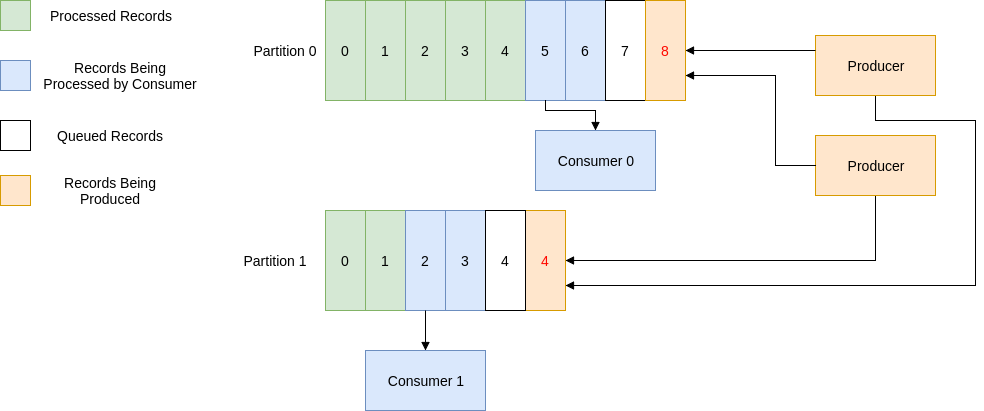
\includegraphics[width=\textwidth]{renders/Kafka.png}
      \caption{Kafka Producers and Consumers}
      \label{fig:kafka}
\end{figure}  

The current situation is outlined as follows:
\begin{itemize}
\item{Consumer 0 has successfully processed (and committed) messages 0 to 4 and is currently processing messages 5 and 6 of partition 0}
\item{Consumer 1 has successfully processed (and committed) messages 0 and 1 and is currently processing messages 2 and 3 of partition 1}
\item{Message 7 in partition 0 and message 4 in partition 1 have both been successfully produced and committed to the log, but not yet processed}
\item{Message 8 in partition 0 and message 4 in partition 1 will be the next messages produced by the producers.}
\end{itemize}

The main purpose of Kafka partitions is to allow records on a single topic to be processed in parallel. As each partition is only owned by a single consumer, the model required for keeping track of what messages have been processed in a certain partition is very simple. However since a consumer may own multiple partitions, the configuration can be tweaked to ensure consumers are always busy. Partitions also aid in keeping records on a single partition isolated. If a bad record appears in a particular partition and the consumer gets stuck trying to process it, only that partition will be impacted.

Each message published to a Kafka partition gets an incremental id known as an \textit{offset}. Consumers are responsible for managing their offset in the message stream. Thus, consumers can be configured to start from any offset, which can even allow for reprocessing of data should the need arise. This has been useful in the past at HubSpot when a bug has caused emails to fail to send. The consumers can have their offsets reset to when the bug first surfaced and the emails will be resent. However this is a delicate process and is only used as a last resort. The offsets for consumers 0 and 1 in \reffig{fig:kafka} would be 4 and 1 respectively.

A key concept to understand about Kafka is that consumers are presented with batches of records, of a configurable size. The batch size in \reffig{fig:kafka} is two. The records inside the batch may be processed out of order, but the batch of records is considered completed \textbf{only when every record in the batch has been processed}. In Kafka, only an entire batch of messages can be marked as processed. For example consider consumer 1 in \reffig{fig:kafka}. Should the consumer succeed to process message two, but fail to process message three, Kafka must be notified of the failure to process the batch of messages (or will notice a timeout) and the entire batch will be retried.


Another interesting concept in Kafka is consumer groups. Consider the case where two entirely separate sets of consumers (running different code) need to read from the same Kafka topic. Both sets of consumers should be able to process every message that is published to the topic and this is what consumer groups provides. Without consumer groups, another consumer could be set up in order to read from the Kafka topic, but as discussed, it would only acquire a certain number of partitions and thus miss some messages (and steal messages from existing consumers). The solution is to specify the consumer group that each running consumer belongs to. In this case, since there are two sets of consumers, both doing different things, there should be two consumer groups. Kafka will then treat all the consumers in each consumer group as if there are no other sets of consumers reading from the Kafka topic. This feature is best understood by considering the two edge cases:

\begin{itemize}
\item{If all consumers are in the \textit{same} consumer group, Kafka simply load balances the partitions across the number of consumers}. Each consumer will see a \textit{subset} of the records published to the Kafka topic, depending on the partitions owned.
\item{If all consumers are in \textit{different} consumer groups, each consumer will have its own offset in \textbf{all} of the partitions. That is, the consumer responsible for partition zero in consumer group A may have a current offset of 100, while the consumer responsible for partition zero in consumer group B may have a current offset of 0. This is essentially, publish-subscribe (pub-sub) behavior. All the consumers will simply see all the records and the rate of consumption of a certain consumer has no impact on the rate of consumption of another consumer.}
\end{itemize}

Continuing with the previous example of having all the emails to be sent through HubSpot contained on a Kafka topic, the following consumer groups could be set up in order to both send every email that appears on the topic and to bill the customer for each email they send. This is shown in \reffig{fig:consumerGroups}
\begin{labeling}{Sending CG}
\item[Sending CG]{This consumer group would contain all the \team{} team's consumers. There would likely be a lot of consumers in this consumer group in order to keep up with the time consuming process of actually sending the emails on behalf of the customers. These consumers would need to be as efficient as possible and the delta between the current offset (the index of the most recently produced message) and the oldest offset (the index of the oldest message still being processed) for each partition would likely be carefully monitored to ensure the consumers are not falling behind}
\item[Billing CG]{This consumer group would perhaps simply read the account number of the customer sending the email and bill that customer. This consumer group would be considerably less time critical and would likely only need to perform some light weight task for each message on the Kafka topic.}
\end{labeling}


\begin{figure}[H]
      \centering
      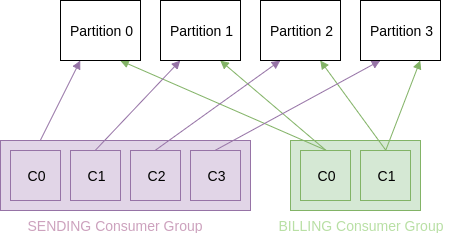
\includegraphics[width=0.6\textwidth]{renders/ConsumerGroups.png}
      \caption{Partition Assignments with Multiple Consumer Groups}
      \label{fig:consumerGroups}
\end{figure}  

A final note of interest regarding Kafka is that it provides an \textit{at-least-once} guarantee that messages will arrive at consumers for processing. If a single message in a batch of messages cannot be processed for whatever reason, the entire batch will be retried. Thus, external idempotency logic is required in order to obtain an \textit{exactly-once} processing guarantee. The \team{} team uses a simple HBase table in order to lock each email that is to be sent, prior to actually sending it. 

\subsection{Hadoop - Big Data Processing}\label{sec:hadoop}
 As with most modern companies, HubSpot's platform generates a monumental amount of data. This data can be leveraged to gain extremely useful insights into how the platform is used, how certain systems are performing and what should be targeted by engineers working on the product. As discussed in \refsec{sec:kafka}, Kafka is used throughout HubSpot to provide high performance data streams. This is ideal for things like moving an email through the entire pipeline from design to sending. However, the contents of Kafka topics are often also persisted (for example for 30 days) to Amazon Web Service's cloud storage facility, Amazon S3 \cite{s3} . Persisted Kafka topics provide a huge amount of data which is typically critical to a system's operations if Kafka is used in the first place. 
 
 Hadoop is a framework that allows for the distributed processing of large data sets across clusters of computers using simple programming models \cite{hadoop}. Often times the size of the datasets persisted to S3 would be too large to hold on disk of a typical machine, and certainly not in memory. Hadoop is horizontally scalable allowing for more and more machines to be added to a cluster as demand grows. Hadoop is used extensively at HubSpot for processing these huge volumes of data by writing Hadoop jobs. These are jobs which make use of the Hadoop framework and run on a cluster created specifically for Hadoop jobs. These jobs can be scheduled and used to periodically hydrate some other data store, or on demand and used when a certain question needs to be answered. 
 
 An example of a scheduled job used by the \team{} team is one which aggregates all the sending statistics for a given HubSpot email sending account. This is used to hydrate an SQL table, which backs an internal dashboard which is used to gain insights into the system. Large customers can potentially send hundreds of thousands, or occasionally millions, of emails in a given day. As discussed, all these emails are contained in Kafka and persisted to S3. In order to extract the useful information, these files need to be indexed and aggregated. Several key values can then be derived from this data such as the percentage of emails sent from this account that were delivered first time, the breakdown of the reasons emails sent from this account were rejected (e.g. the IP has a bad reputation) and many others.

Hadoop offers a large number of benefits. Hadoop is fault tolerant - for example if a mapper node dies and produces no output, the corresponding map process will be repeated on another node. Hadoop make use of the \textit{Hadoop Distributed File System (HDFS)} \cite{HDFS} which provides data replication and support for huge datasets. One of the key benefits of using HDFS that Hadoop leverages is that it can attempt to assign work to nodes based on the data they \textbf{already have}. This limits the costly operation of moving data around the network. This is succinctly summarized by Hadoop's famous design ethos - \textit{"bring the processing to the data"}.

The main user facing API contained in Hadoop, is Hadoop Map-Reduce. Map-reduce is a programming model for highly parallelizable data processing. The map-reduce methodology consists of four key phases - \textit{split, map, shuffle, reduce}. As an example, consider a dataset which is a corpus of quotes of the form:
\textit{"Learning never exhausts the mind - Leonardo da Vinci"}. An example task on this dataset would be to calculate the number of quotes contained by each of the authors in the corpus. This would be implemented using map-reduce in the following manner:

\begin{labeling}{Reduce }
	\item [Split] The initial step would be to split the corpus into chunks for processing on different nodes in the cluster. As discussed, Hadoop does this intelligently by trying to assign chunks for processing to worker nodes who already contain that data. This phase would output a single record for each quote in the corpus.
  \item [Map] This is the beginning of the useful processing of the data. The purpose of the map phase is to output a key-value pair. In this example, the key would be the name of the author and the value would simply be one, as each entry in the corpus is a single quote. The map phase would likely require a regular expression to parse the name of the author from the quote.
  \item [Shuffle] The \textit{shuffle} phase is responsible for grouping the output key value pairs produced by the map phase by key. This forms a list of the values that are associated with each key from the map phase. In this example, a possible output of the shuffle phase would be: \java{Leonardo da Vinci -> [1, 1, 1]}, indicating that three entries with the key ``Leonardo da Vinci'' were found and each had a corresponding value of 1. 
  \item [Reduce] The final phase is the \textit{reduce} phase. The input to the reduce phase is the output of the shuffle phase - a key and a collection of values associated with that key. As the name suggests, the reduce phase is responsible for reducing this collection of values down to a single value. In this example, the single value output of the reduce phase would simply be the number of elements in the collection of values, indicating the number of quotes found by the particular author.
\end{labeling}


\subsection{Protobuf - Structured Data Serialization}\label{sec:protobuf}
Protocol Buffers (Protobuf) are Google's language-neutral, platform-neutral, extensible mechanism for serializing structured data \cite{protobuf}. Protobuf is similar in concept to XML or JSON, but produces data which is 3 to 10 times smaller in serialized form \cite{protobufSizeStat}. Protobuf also offers many powerful features such as enums, types, default values and nested messages.

Protobuf works by defining the desired data structures in a special .proto file. Compilers exist for a large number of languages (e.g. Java, C++, Python etc) which compile these .proto files into classes usable inside the language. For example the Java Protobuf compiler generates immutable Java objects with a variety of useful features such as builders and methods for serializing and deserializing to and from immutable byte arrays. The serialization / deserialization process is extremely fast and is especially useful in conjunction with Kafka (see \refsec{sec:kafka}), which operates solely on byte arrays. An example of a Protobuf message for a person is shown in \refcode{lst:protoPerson}. This example shows the rich features such as optional fields (email), enums (PhoneType), nested messages (PhoneNumber) and arrays of values (PhoneNumber).

\lstinputlisting[
  caption={A Protobuf Representation of a Person},
  label={lst:protoPerson},
  style=protoStyle,
  ]{code/technologies/person.proto}

\subsection{gRPC - Remote Procedure Calling}
gRPC is a cross language remote procedure calling framework \cite{gRPC}. It serves as an alternative to the current de facto standard of having services communicate using REST endpoints over HTTP/1.1. gRPC operates by defining a service and specifying the methods that can be called remotely, along with their parameters and return types \cite{gRPCDef}. gRPC uses Protobuf (see \refsec{sec:protobuf}) as its IDL (interface definition language). That is, the defined methods (by default) accept as parameters, and return, Protobuf messages. As with Protobuf, compilers exist for a variety of languages which generate the client side and server side code for their respective languages. Clients of the service can then remotely invoke these methods on objects they hold known as \textit{stubs}. The methods are then remotely invoked on the server. To the client, the procedure call appears no different to any other procedure call as all the remote networking is handled by the framework. 

gRPC is built upon HTTP/2 which offers many new powerful features. One of the main advantages of HTTP/2 over HTTP/1.1 is multiplexing which allows multiple HTTP requests to be made (and responses received) asynchronously over a single TCP connection. The enables the gRPC framework to provide four types of RPC invocations:

\begin{enumerate}
  \item{The first type of call is a simple \textit{unary} call. In this case, the client sends a single request to the server, who handles the request and returns a single response. This is equivalent to a typical HTTP/1.1 request and response.}
  \item{The second type of call is \textit{server side streaming}. In this case, the client sends a single request to the server and the server responds with a stream of messages. This is useful in cases where the response may be a large collection of items. The client may not need \textbf{all} of the items before it can begin processing. Thus, the server can respond with a stream, allowing the client to begin reading messages from the stream as they become available.}
  \item{The third type of call is \textit{client side streaming}. This is the exact opposite to server side streaming and is useful in cases where the client must send a lot of data, but the server can begin processing that data before it has all been received.}
  \item{The final type of call is \textit{bidirectional streaming}. As expected, this is when both the client and server communicate using streams. These streams are entirely independent from one and other, allowing the client / server to read messages in any order.}
\end{enumerate}

The \team{} team uses gRPC at the final stage of the email sending pipeline. The last step is to get the email to the servers which are responsible for sending the email to the recipient using SMTP (see \refsec{sec:smtp}). As discussed in \refsec{sec:emailSendingInfra}, SMTP email sends can take on the order of seconds. This leads to a very asynchronous system which causes issues if using standard REST endpoints over HTTP/1.1. 

gRPC is used in this case instead of Kafka as particular emails \textbf{must} be sent from particular IP addresses for SPF to pass (see \refsec{sec:DNS} for more information on SPF). Certain email sending servers will be bound to certain public IP addresses, meaning certain emails \textbf{must} be sent from certain servers. If Kafka was used for the final step, there is no guarantee that the consumer who owns the partition the email ends up in will be bound to the correct IP address, meaning they would not be able to send the email. gRPC can be used to connect to the server who is \textbf{known} to be bound to the correct IP address. This could also accomplished using a simple REST endpoint, but as discussed, this causes performance issues.

\section{Email Specific Technologies}
\subsection{Domain Name System (DNS)} \label{sec:DNS}

Although not entirely email specific, DNS is extremely critical for the \team{} team. Aside from teams working on the HubSpot development platform (that is teams working on the platform which engineers develop HubSpot products on), most other teams need not concern themselves with DNS at all. However as DNS is such an important component of email, DNS records must be carefully maintained. For email, there are five key DNS record types, outlined below.

\begin{labeling}{DKIM }
  \item[A] A records are used extensively in DNS. These records define the IP address that is associated with a particular domain. For example, the IP address of the web server which hosts the website \textit{hubspot.com} can be obtained by performing a DNS lookup for the A record associated with \textit{hubspot.com}. This address translation is done every time a user visits a website and enables the use of memorable, human friendly domain names instead of raw IP addresses.
  \item[MX] MX (Mail Exchanger) records are similar to A records except they define the \textbf{hosts} which can accept mail for a given domain. For example, if an email is to be sent to \textit{billing@hubspot.com}, the email sender must know where to send that email. Thus, an MX lookup is performed for \textit{hubspot.com}, the domain in which the account associated with the email address \textit{billing@hubspot.com} resides on. This typically returns a host name, for example, \textit{mx.hubspot.com}. Thus, a subsequent A record lookup for \textit{mx.hubspot.com} is required to determine the exact IP address(es) of the server(s) which can accept email for \textit{billing@hubspot.com}.
  \item[SPF] SPF (Sender Policy Framework) records are used to authorize a set of IP addresses which a domain intends to send email from. The friendly-from address of an email (the sender's address) is simply a plain text header contained in the email. This means that anyone could potentially send email as someone else by spoofing the friendly-from address. SPF records provide part of the mechanism which solves this problem. A domain can declare a list of IP addresses it intends to send email from using an SPF record. Thus, when an email is received from \textit{stefano@example.com}, the SPF record associated with \textit{example.com} can then be fetched and if the source IP address of the email does not match one of the declared IP addresses, the email may be blindly accepted, tentatively accepted or dropped entirely. An example SPF record would be \java{v=spf1 ip4:1.2.3.4/30 -all}. The first component (\java{v=spf1}) indicates the SPF version in use, the second component (\java{ip4:1.2.3.4/30}) is a CIDR representation of the IP addresses this domain authorizes (see \refsec{sec:CIDR}) and the final component (\java{-all}) indicates that email sent from all other IP addresses except the ones defined here should be dropped. 
  \item[PTR] PTR records are the inverse of A records and are used to determine the host associated with a particular IP address. 
  \item[DKIM] DKIM (DomainKeys Identified Mail) records provide another level of authentication. DKIM uses asymmetric-key cryptography to digitally sign emails, verifying that the email was sent by an authorized sender (provided only authorized senders hold the private key). The public component of DKIM keys are contained under the \java{_domainkey} sub domain and are prepended with a DKIM \textit{selector} indicating which DKIM key was used. The \textit{DKIM-Signature} header is included in the email, an example of which is shown in \refcode{lst:dkimSig}.
  \lstinputlisting[
  caption={An Example DKIM signature},
  label={lst:dkimSig},
  style=protoStyle,
  ]{code/technologies/dkim.txt}

  The most important DKIM tag-value pairs are outlined below \cite{dkimSig}:
  \begin{labeling}{bh }
    \item[v] This indicates the DKIM version in use
    \item[a] This indicates the algorithm used to generate the signature.
    \item[s] This is the selector prefix and is used to pick the public key to use from those available at the \java{_domainkey} subdomain.
    \item[h] This contains the list of headers which were hashed to generate the \textit{b} tag
    \item[b] This contains the Base-64 encoded hash of the headers listed in \textit{h}
    \item[bh] This contains the hash of the body of the email
    \item[d] This contains the domain in which the corresponding public key can be found
  \end{labeling}

  The corresponding public key can be found by performing a TXT lookup of \java{<s>._domainkey.<d>}, or in the above case \java{dk1._domainkey.example.com}. The value of these records also contain tag-value pairs, such as \textit{k} which indicates the cryptography system used and \textit{p} which contains the public key itself. Once the public key has been obtained, the inverse of the signing operation can be applied to ensure the email came from an authorized sender.
\end{labeling}


\subsection{Simple Mail Transfer Protocol (SMTP)} \label{sec:smtp}
SMTP is the protocol used for sending email to a mail server. SMTP is quite an old protocol, with the first RFC being published in 1982 \cite{smtpRfc}. For an email to be sent from one machine to another, a connection must be opened up between the mail server responsible for the sender's email and the mail server responsible for the recipient's email. SMTP defines the way in which messages should be exchanged between these two servers. Most mail servers today support 
Extended SMTP (ESMTP), which is outlined in RFC 1869 \cite{esmtpRfc}. This defines a format for indicating which extensions a given SMTP server supports. 

SMTP contains 6 main steps to send email:
\begin{labeling}{MAIL FROM: }
  \item[EHLO] The first SMTP command of interest is \java{EHLO <SMTP domain>}. This is the first message expected by the server. In turn, the SMTP server will respond with a 250 OK message and list all the extensions it supports. 
  \item[MAIL FROM:] The sender then specifies the mail from address to be used for the email (who the email was sent from) using \java{MAIL FROM: <from_email_address>}. Again, provided the server accepts the email address as valid, the server should return a 250 OK.
  \item[RCPT TO:] The sender then specifies the email address that the SMTP server should deliver the email to using \java{RCPT TO: <recipient_email_address>}. Provided the SMTP server accepts responsibility for this recipient address (it expects to receive email for this address), the server will again respond with a 250 OK. Otherwise, the server will reject the message and terminate the connection.
  \item[DATA] The sender then indicates that it wishes to begin sending the data contained in the email message, by sending the \java{DATA} command. The server will then return with a 354, along with some instruction on how to terminate the message, indicating that the client may begin to send the message.
  \item[<content>] The sender then proceeds to send the content of the email message line by line, followed finally by a specific message indicating that the content is completed. This termination message is a single period character on its own line. The server should again respond with a 250 OK once the content has been received.
  \item[QUIT] Finally, the sender issues a \java{QUIT} command. The server will respond with a 221 message and the session may be safely terminated.
\end{labeling}

As the name suggests, SMTP is quite a simple protocol. Many libraries exist which handle SMTP messaging exchanges. However as this needs to happen for every single email that is sent through HubSpot, the \team{} team implemented their own Java high performance and open source SMTP library, NioSmtpClient \cite{hubspotSmtp}. This SMTP client supports several of the SMTP extensions such as TLS which provides encryption and SMTPUTF 8 which supports sending UTF8 characters over SMTP. It also allows connections to be recycled and can automatically determine most efficient sending method based on the EHLO response from the server.     

\section{System Management and Health Monitoring}
While working on projects of this magnitude, bugs and issues are an inevitability. The amount of traffic seen by these systems compounds any small issues or bugs present in the system. As such, it is critical to have systems in place which monitor the health of the system and inform the team of any potential issues with the system. What's more, these issues must be continuously examined and remedial action must be taken where applicable. The \team{} team makes use of several tools and methods for monitoring the health of their systems, a subset of which are outlined in the following sections.

\subsection{Log4j2}\label{sec:log4j2}
Log4j2 \cite{log4j2} is a Java framework which is provides facilities for logging to different log levels and advanced log filtering (for example with regular expressions). This provides an excellent facility for understanding why systems are behaving unexpectedly in production. A common pattern is to insert log messages to a low priority log level (e.g. DEBUG) which describe the state of the system or the code path taken. Typically, when the system is behaving normally, a higher priority log level is set (e.g. INFO) meaning these finer grained log messages are skipped. However, should an issue arise, the log level can then be easily switched to the lower priority temporarily to get a more detailed insight into why the system is misbehaving. This pattern allows detailed log messages to be produced only when they are needed, reducing the amount of noise present in the logs. The framework also provides the ERROR level which can log error messages as uncaught exceptions without killing the currently executing thread.

\subsection{Sentry}
Sentry \cite{sentry} is an online platform which logs uncaught exceptions that arise during program execution. This greatly simplifies the task of finding out the reason for a system fault or failure without the need to trawl through pages of log files. Sentry logs the full stack trace associated with an exception, the time of occurrence and other pieces of metadata such as the name of the deployable. It uses this data to monitor the occurrences of particular exceptions over time, provides facilities for opening and closing GitHub issues and most importantly, to send an email to all those subscribed to the project (e.g. the \team{} team in this case) when an exception occurs. Sentry proves to be extremely useful at deploy time. Obviously when deploying new code to production servers, one must be sure that the changes did not cause the system to enter an unhealthy state. Provided the code is well written and that unexpected exceptions that occur are not silently swallowed, Sentry can be monitored at deploy time in order to help provide the engineer with confidence that the deployed changes were non breaking. Sentry also provides support for integrating into Log4j2 (see \refsec{sec:log4j2}). Sentry can monitor ERROR level log messages that are produced by Log4j2 and subsequently log these error messages to the Sentry platform. As an engineer this combination of tools is extremely useful for indicating that the system has found an issue, without killing the thread. This is ideal in cases where some work has been done and the system has encountered a critical error, but does not need to be restarted. This mitigates the need to repeat the work, but still informs the team that an error has occurred by logging an exception to Sentry.

\subsection{SignalFX}
SignalFX \cite{sigfx} is an online tool for recording metrics and data visualization. Gathering and analysing metrics is a key part of ensuring the health of a complex system. When things start to fail, SignalFX is the first place engineers look to. SignalFX essentially allows data to be dumped to the cloud and for complex graphs and charts to be rendered in real time using this data. SignalFX supports creating dashboards consisting of many of these graphs and charts. The \team{} team has several of these dashboards, each encapsulating a single part of the system. When problems inevitably arise, the team can examine these dashboards in order to try to isolate and find the problem. Once remedial action has been taken, the dashboards can be monitored to ensure the desired effect takes place. Being able to see these metrics in close to real time is incredibly useful for diagnosing faults with the system. It also serves as an excellent mechanism for finding parts of the system that can be improved. For example, critical code paths can be timed and the results logged to SignalFX. This allows accurate inferences to be made about parts of the system and allows the team to target parts of the system which need improvement.

SignalFX also allows for detectors to be configured. For example, a chart could be created monitoring the number of emails sent in the past minute by each IP address responsible for sending emails. A detector can then be put in place to detect if this number falls below a certain threshold. Detectors can be configured to alert via email and Slack when they trigger, allowing engineers to be notified. 

SignalFX also supports complex data aggregations. This is beneficial as it decouples calculations that need to be done on metrics from the code which the metrics are monitoring. Performing any sort of data manipulation in performance critical code paths is obviously not desirable when every millisecond counts. Instead, metrics gathering is as simple as producing the data to SignalFX. The complex graphs and charts can then be configured inside of the SignalFX tool, entirely independent to the production code. 